%%==================================================
%% chapter01.tex for BIT Master Thesis
%% modified by yang yating
%% version: 0.1
%% last update: Dec 25th, 2016
%%==================================================
\chapter{绪论}
\enchapter{Introduction}
\label{chap:intro}
\section{研究背景及选题意义}
\ensection{Research Background and Motivation}

\subsection{研究背景}
\ensection{Research Background}

无服务器计算已成为当今云和数据中心基础架构的新兴范式。 它使用一种单点服务或功能作为基本计算单元,该单元以多种方式轻松计算。 首先,它可以帮助应用程序开发人员专注于核心逻辑,并将与基础架构相关的任务(例如自动缩放)留在无服务器平台上。 其次,它采用了具有细粒度付费模式(例如1MS [7])的pay-as-you-go模型,以便用户可以节省未使用的计算资源的成本。 第三,无服务器计算也使云提供商有益于他们可以更有效地管理资源。Serverless的核心思想是将基础设施的管理责任交给云服务提供商,用户无需关心服务器的配置和管理,可以专注于业务逻辑的实现。然而,在Serverless环境中,如何高效、安全地运行容器化应用仍然是一个亟待解决的关键问题。


容器技术作为现代云计算架构的重要组成部分,广泛应用于Serverless平台中。容器通过提供轻量级的隔离和高效的资源利用,为应用的部署和弹性伸缩提供了便利。在Serverless平台上,容器化应用需要支持快速启动和高并发运行,这对容器管理系统的性能和可扩展性提出了更高的要求。Linux内核中的cgroup(控制组)机制是容器资源管理的基础,它提供了对容器资源(如CPU、内存、网络带宽等)的隔离和限制。然而,现有cgroup机制在面对高并发、大规模容器启动的场景时,仍然存在性能瓶颈和可扩展性问题,亟需进行优化。

另一方面,eBPF(扩展的伯克利包过滤器)作为Linux内核的一项强大特性,已在网络、安全、性能监控等多个领域得到了广泛应用。eBPF允许在内核中运行用户定义的程序,极大地扩展了内核的功能。eBPF Verifier作为eBPF框架的一部分,主要用于在编译时静态检查eBPF程序的正确性和安全性,确保程序在运行时不会导致系统不稳定或安全漏洞。

此外,随着数据处理能力的提升,异构计算平台(如集成了DPU的服务器)在云计算中逐渐得到广泛应用。DPU(Data Processing Unit)作为一种专为数据处理优化的计算单元,可以显著提升网络处理、存储加速等方面的性能。然而,Serverless平台中使用DPU加速计算时,如何确保多租户环境下的安全性,尤其是不同租户间对DPU资源的隔离,成为了一个重要问题。为了解决这一问题,利用静态程序验证技术(如eBPF verifier)来分析和保证代码的安全性和隔离性,成为了一个有效的解决方案。

\subsection{选题意义}
\ensection{Motivation}
本研究的主要目标是提升Serverless环境中容器应用的安全性和性能,尤其是在异构计算平台下。研究的意义可从以下几个方面进行阐述:

优化cgroup机制提升并发启动性能
随着Serverless架构的广泛应用,容器化的应用需要在高度动态和弹性的环境中快速启动和运行。Linux内核的cgroup机制在容器的资源管理和隔离方面发挥了重要作用,但在面对高并发容器启动时,现有cgroup的性能和可扩展性仍然不足。通过对cgroup机制进行优化,可以有效提升Serverless平台中容器的启动效率,增强平台在高并发环境下的稳定性和扩展能力,满足现代云计算平台对高性能和高并发的需求。

保证DPU资源的安全隔离
在Serverless环境中,DPU作为一种硬件加速单元,可以显著提升计算效率。然而,DPU作为共享资源在多租户环境中的使用,容易面临安全性和资源隔离的问题。如何保证不同租户在使用DPU时的资源隔离性,防止不同租户之间相互干扰,成为了一个亟待解决的难题。本研究通过引入类似eBPF verifier的静态程序验证技术,能够在运行时前对DPU访问代码进行验证,确保多租户环境下对DPU的安全访问,从而避免内存泄露、数据篡改等安全风险。

推动Serverless平台在异构计算环境中的应用发展
目前,Serverless架构的研究主要集中在通用的计算资源和虚拟化技术上,针对异构计算资源(如DPU、GPU等)的支持尚处于起步阶段。本研究不仅将研究如何在Serverless架构中高效、安全地使用DPU加速计算,还将探索如何使Serverless平台更好地适应异构计算环境,为异构计算资源的全面融合提供理论依据和技术支持。

促进Serverless技术的商业应用和发展
随着云计算技术的不断发展,Serverless架构在互联网企业和各类业务应用中的应用越来越广泛。通过提升Serverless平台在高并发、大规模容器管理和异构计算资源安全管理方面的能力,本研究的成果不仅具有重要的学术价值,同时对促进Serverless技术在商业应用中的推广和发展具有重要意义。

\captionsetup[figure]{justification=justified}
\begin{figure}
	\centering
		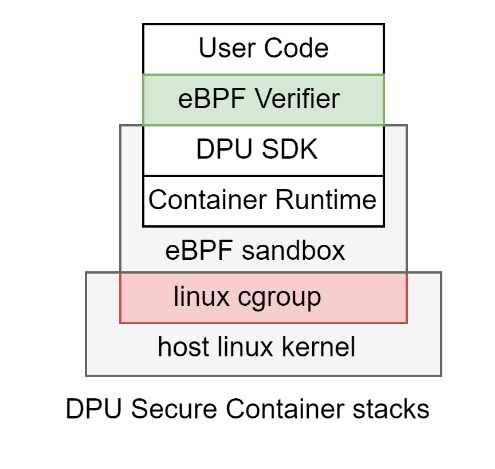
\includegraphics[width=0.4\textwidth]{figures/figure0}
 \label{fig:Overview-1}
 \caption{Overview}
\end{figure}


\subsection{研究目标和内容}
\ensection{Research objectives and content}
本论文的主要研究目标是通过优化Linux内核cgroup机制,提高Serverless环境下容器的并发启动性能;通过引入静态程序验证技术,保证Serverless平台中DPU资源的多租户安全隔离。具体内容包括:

优化cgroup机制:研究并优化Linux cgroup在高并发、大规模容器启动场景中的性能瓶颈,提高其在Serverless环境中的可扩展性和响应速度。
eBPF验证技术的应用:通过引入eBPF verifier等静态验证技术,确保Serverless平台中异构计算资源(如DPU)的安全隔离,避免不同租户间的资源竞争和安全问题。
通过以上研究,本论文旨在为异构计算平台下的Serverless架构提供高效、安全的容器应用加速技术,为下一代云计算平台的发展做出贡献。

\section{国内外研究现状}
\ensection{Research Progress Overview in Home and Abroad}
%\label{sec:***} 可标注label

\section{本文主要内容和章节安排}
\ensection{Major Contents and Chapter Arrangement}

%\label{sec:features}





\subsection{Serverless 函数并发启动关键技术点}
%\label{sec:requirements}

\subsection{基于eBPF的DPU静态虚拟化}

云计算技术对异构需求越来越高,传统架构存在着处理能力与数据量增长不匹配、资源利用不足、安全风险等问题。DPU功能serverless化变得非常常见。例如英伟达推出的DOCA平台框架(DPF)是一个DPU程序编排框架,帮助创建BlueField加速的云软件平台,使得DPU可以在K8s环境中被直接使用。同时已有研究人员开始研究异构计算系统(CPU-GPU-DPU)上的serverless系统(Serverless Computing on Heterogeneous Computers ASPLOS’22)。

DPU 容器(DPU container)通常是指基于 DPU(数据处理单元)技术,使用容器化技术来部署和管理的计算环境。简单来说,它结合了 DPU 的硬件加速能力和容器的灵活性,通常用于高性能计算、网络加速、存储加速等场景。
Nvidia DPU具有硬件级隔离:NVIDIA BlueField DPU通过硬件加速引擎和专用处理资源,为每个租户提供独立的计算、存储和网络资源,确保租户之间的资源隔离。在云原生计算平台中,DPU通过卸载和加速基础设施功能,支持多租户环境下的高性能计算。DOCA编程框架(DPF)可以实现多租户的DPU服务的调配和编排,通过容器化的方式将 Kubernetes 控制平面功能扩展到 DPU,使管理员能够直接在 BlueField DPU 上部署和卸载 NVIDIA DOCA 服务和基于 DOCA 的第三方服务。DPF 配备了专门用于无缝集成的 SDK,提供了一个一致的模块化工具包,例如OVS,RDMA开发工具包。

\captionsetup[figure]{justification=justified}
\begin{figure}
	\centering
		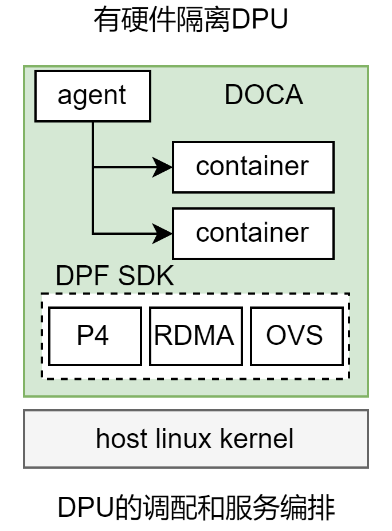
\includegraphics[width=0.3\textwidth]{figures/figure2}
 \label{fig:diagram}
 \caption{DPU 应用程序的调配和服务编排}
 
%  \captionwithsource{热塑性形状记忆聚氨酯的形状记忆机理示意图}{数据来源:交代图形的出处或者来源,示明“作者、来源名称、时间”,用小五宋体,置图左下方。交代图形的出处或者来源,示明“作者、来源名称、时间”,用小五宋体,置图左下方。}
\end{figure}

目前国内的 DPU(数据处理单元)在硬件级隔离方面的能力相对有限,要实现完全的硬件级隔离(特别是在安全性、可靠性、性能等方面的完全隔离)仍需要进一步的技术发展和硬件支持,尤其是是在K8s等云应用场景下。

1.虚拟化和资源隔离:许多 DPU 提供了硬件加速的虚拟化支持,尤其是在网络、存储和计算资源的隔离方面。例如,DPUs 如浪潮的“云脉”DPU或者华为的“昇腾”DPU,已经具备一定的隔离能力,能够在同一物理硬件上支持多个虚拟机或容器的运行,并为其提供网络加速、存储加速等服务。但这种隔离更多是针对资源访问的虚拟化层面的,而非完全的硬件隔离。

2.安全性与可信计算:要实现完全的硬件级隔离,还需要依赖于更强的安全特性,比如硬件级的加密、完整性保护、物理隔离等机制。目前一些 DPU 已经支持基于硬件的安全功能(如加密引擎),但对于极高要求的安全场景(如政府、金融等领域),硬件级的完全隔离通常需要结合特殊的硬件设计和安全协议,甚至依赖于可信执行环境(TEE)技术。

3.DPU与CPU的协同工作:目前的 DPU 在硬件级的完全隔离方面,可能仍然受到 CPU 和内存共享、I/O 访问控制等因素的制约。尤其是在一些复杂的并发计算和高性能计算场景下,虽然 DPU 可以通过硬件支持高效的网络处理和计算加速,但要完全独立于 CPU 的安全和资源调度依然是一个技术难点。

目前国内的这种不具备完全硬件隔离能力的DPU无法支持租户之间的资源隔离要求,阻碍了DPU容器化的应用。
ebpf 借助ebpf verfier实现了一个安全的沙箱,可以防止ebpf代码以多种方式来损害内核(DOS攻击、信息窃取攻击等)。Verifier可以在一定程度上对容器内的代码实现安全性隔离(todo:需要找一些case分析)。同时,eBPF verifier运行在程序加载阶段,不会给函数容器启动添加额外影响。 通过ebpf verifier实现ebpf sandbox可以在软件层面对用户代码实现安全保障作用。加入ebpf sandbox后的DPU容器化模型如下图所示:

\captionsetup[figure]{justification=justified}
\begin{figure}
	\centering
		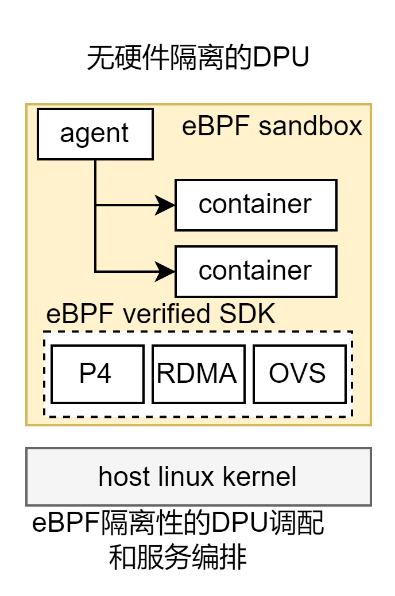
\includegraphics[width=0.3\textwidth]{figures/figure3}
 \label{fig:diagram}
 \caption{eBPF隔离的DPU调配和服务编排}
 
\end{figure}

1. 硬件虚拟化与资源分区
SR-IOV(单根I/O虚拟化)
DPU的物理网卡通过SR-IOV虚拟化为多个虚拟功能(VF),每个租户的虚拟机(VM)或容器独占一个VF,实现网络流量的直接硬件隔离,减少延迟并提升吞吐量。

硬件资源分片
DPU的计算核心(如Arm CPU、加速引擎)和内存资源通过硬件分区分片,为不同租户分配独立的计算单元和内存空间,防止资源争用。